%%%%%%%%%%%%%%%%%%%%%%%%%%%%%%%%%%%%%%%%%%%%%%%%%%%%%%%%%%%%%%%%%%%
%%%%%%%%%%%%%%%%%%%%%%%%%  LAUNCHING SYSTEM  %%%%%%%%%%%%%%%%%%%%%%%%%%%%%
%%%%%%%%%%%%%%%%%%%%%%%%%%%%%%%%%%%%%%%%%%%%%%%%%%%%%%%%%%%%%%%%%%%
%%%%%%% PRIMERA LLISTA DE CANDIDATS: PRIMER PARAGRAF DE LAUNCH SITE AND VEHICLE ANALYSIS %%%%%%%
The following table displays the first seven candidates. 
\newline	
	\begin{table}[h]
	\begin{center}
	\begin{tabular}{|c|c|c|c|}
	\hline
	\bf{ENTERPRISE} & \bf{ROCKET} & \bf{LAUNCHING SITE} & \bf{TYPE}  \\
	\hline 
	Rocket Labs & Electron & North Island (New Zealand) & Light \\
	\hline 
	Kosmostras & Dpner & Baikonur Cosmodrome (Kazakhstan) & Light\\
	\hline 
	Arianespace & Ariane V & Guiana Space Center (French Guiana) & Heavy \\
	\hline
	 Arianespace & Vega & Guiana Space Center (French Guiana) & Light\\
	\hline 
	SapceX & Falcon 9 & USA & Heavy \\
	\hline 
	PLDSpace & ARION-2 & Huelva and Cape Canaveral & Light\\
	\hline 
	LEO Launch and Logistics & - & USA & Light \\
	\hline
	\end{tabular}
	\end{center}
	\caption{List of Launchers}
	\end{table} 
%%%%%%% ELECTRON %%%%%%%
\newline
\begin{figure}[h!]
\centering 
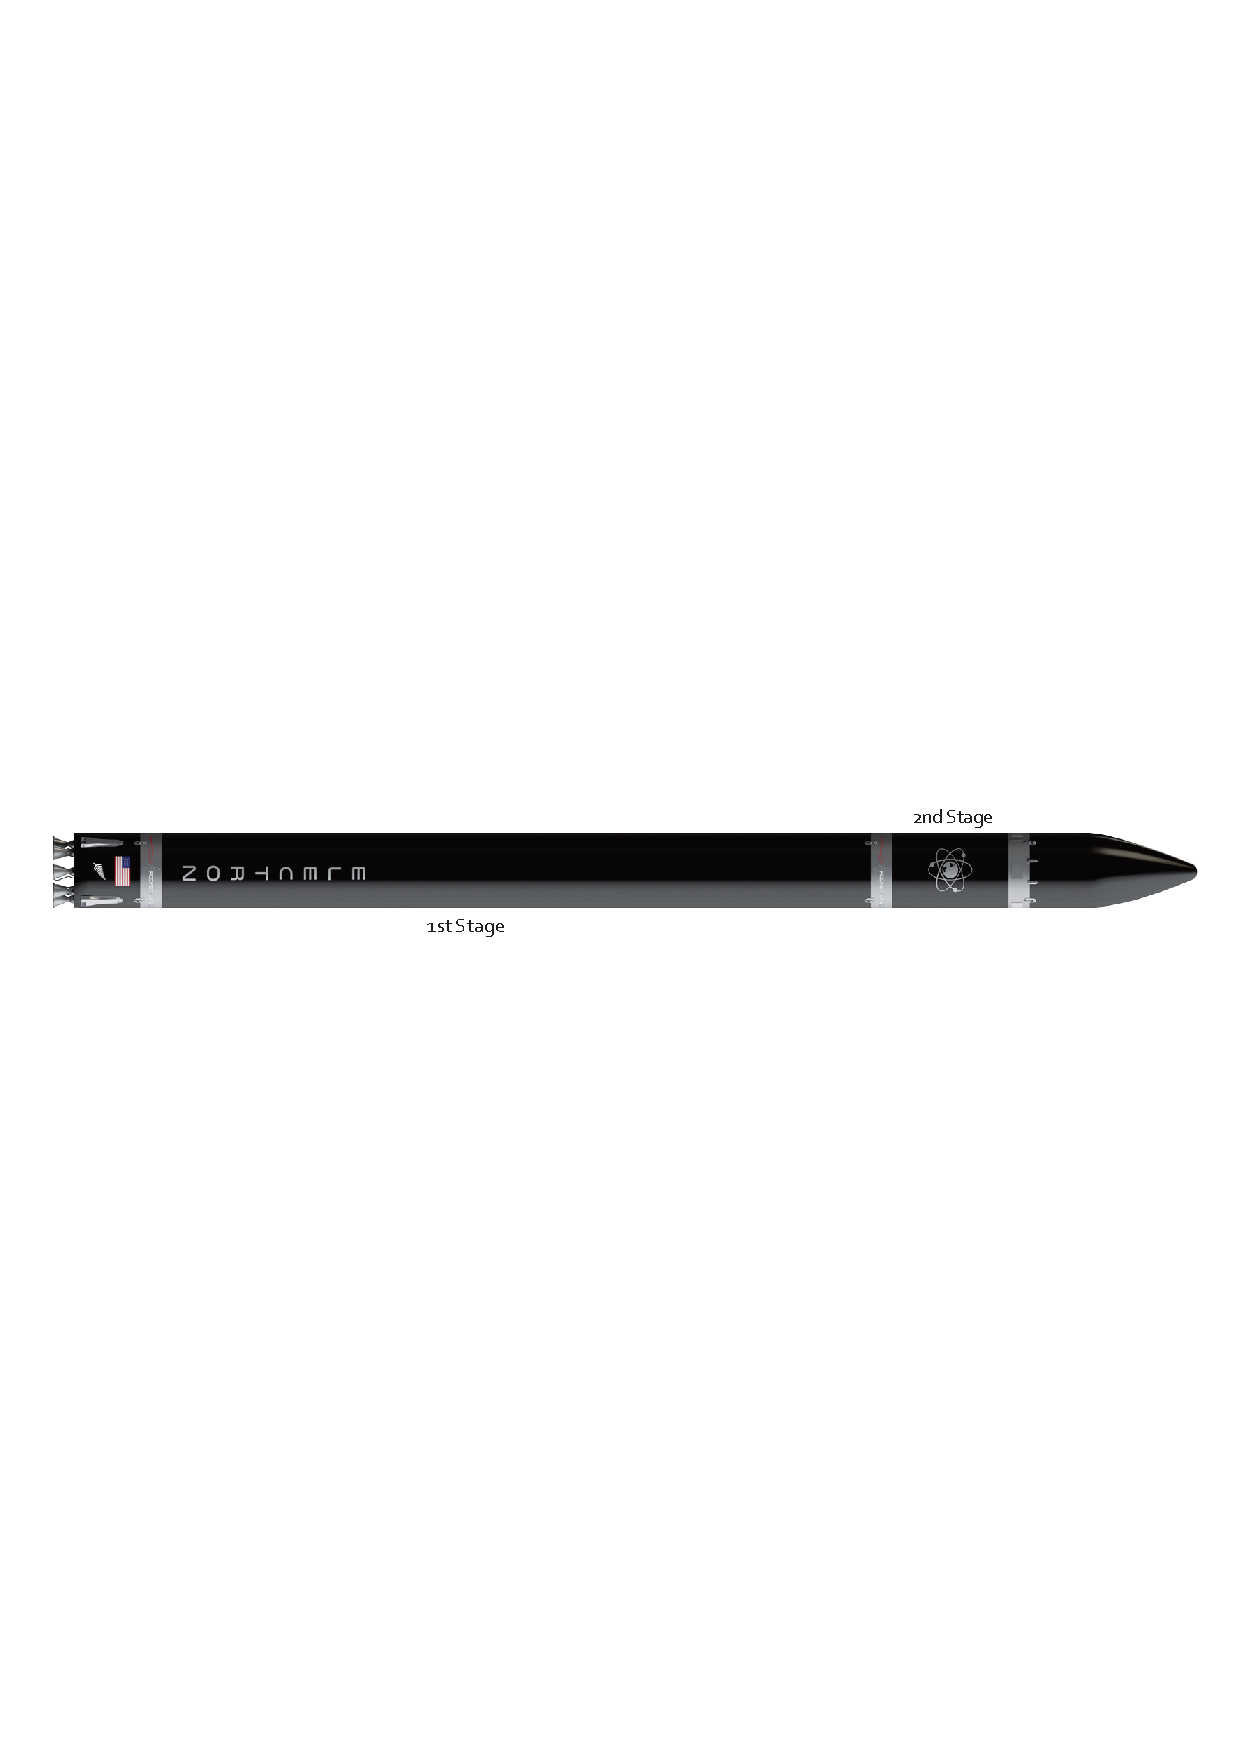
\includegraphics[scale=0.7]{./sections/Constellation_Deployment/S2-Launcher/Images_S2/Picture_1_S2.pdf} 
\caption{Electron Rocket}
\label{fig:rocket}
\end{figure}
\newline\newline
\begin{figure}[h!]
\centering 
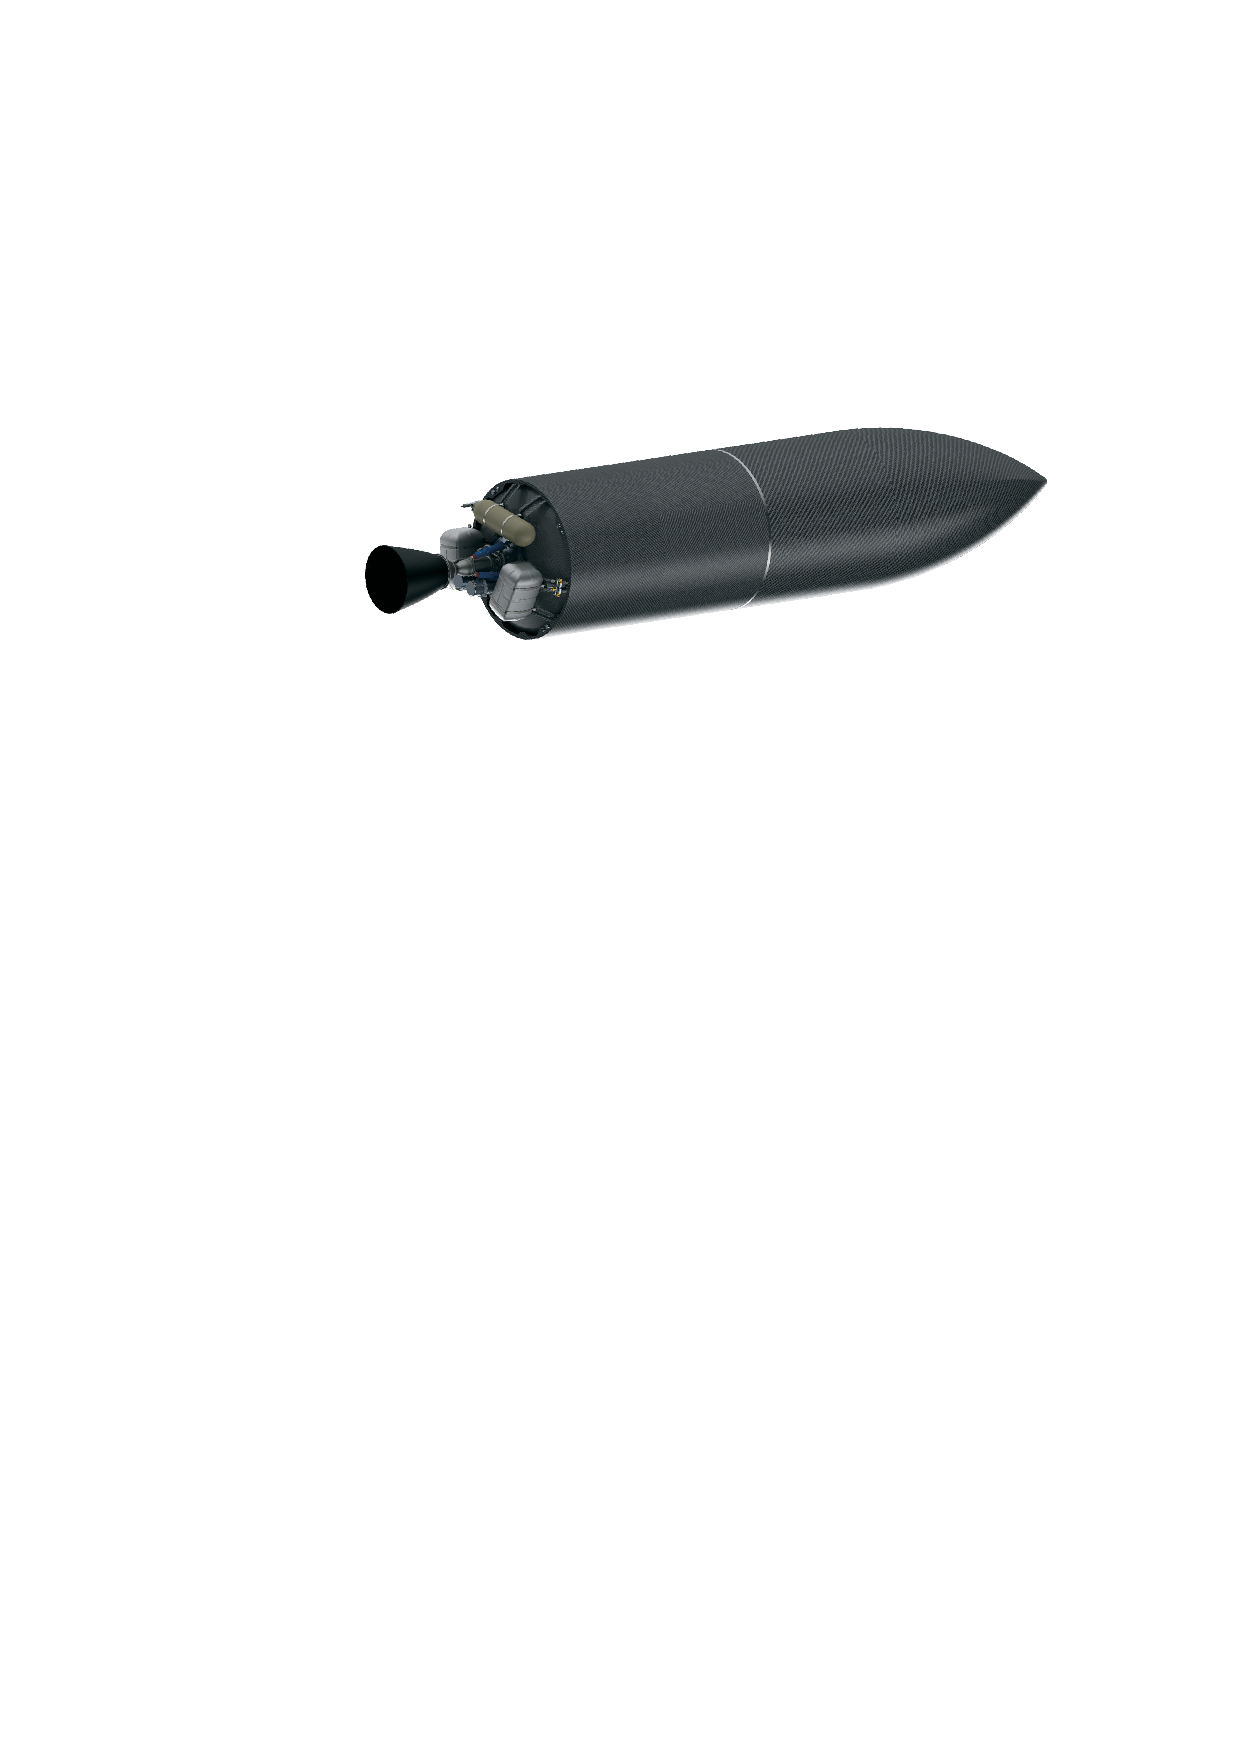
\includegraphics[scale=0.6]{./sections/Constellation_Deployment/S2-Launcher/Images_S2/Picture_2_S2.pdf} 
\caption{Second Stage}
\label{fig:second}
\end{figure}
\newline\newline
\begin{figure}[h]
\centering 
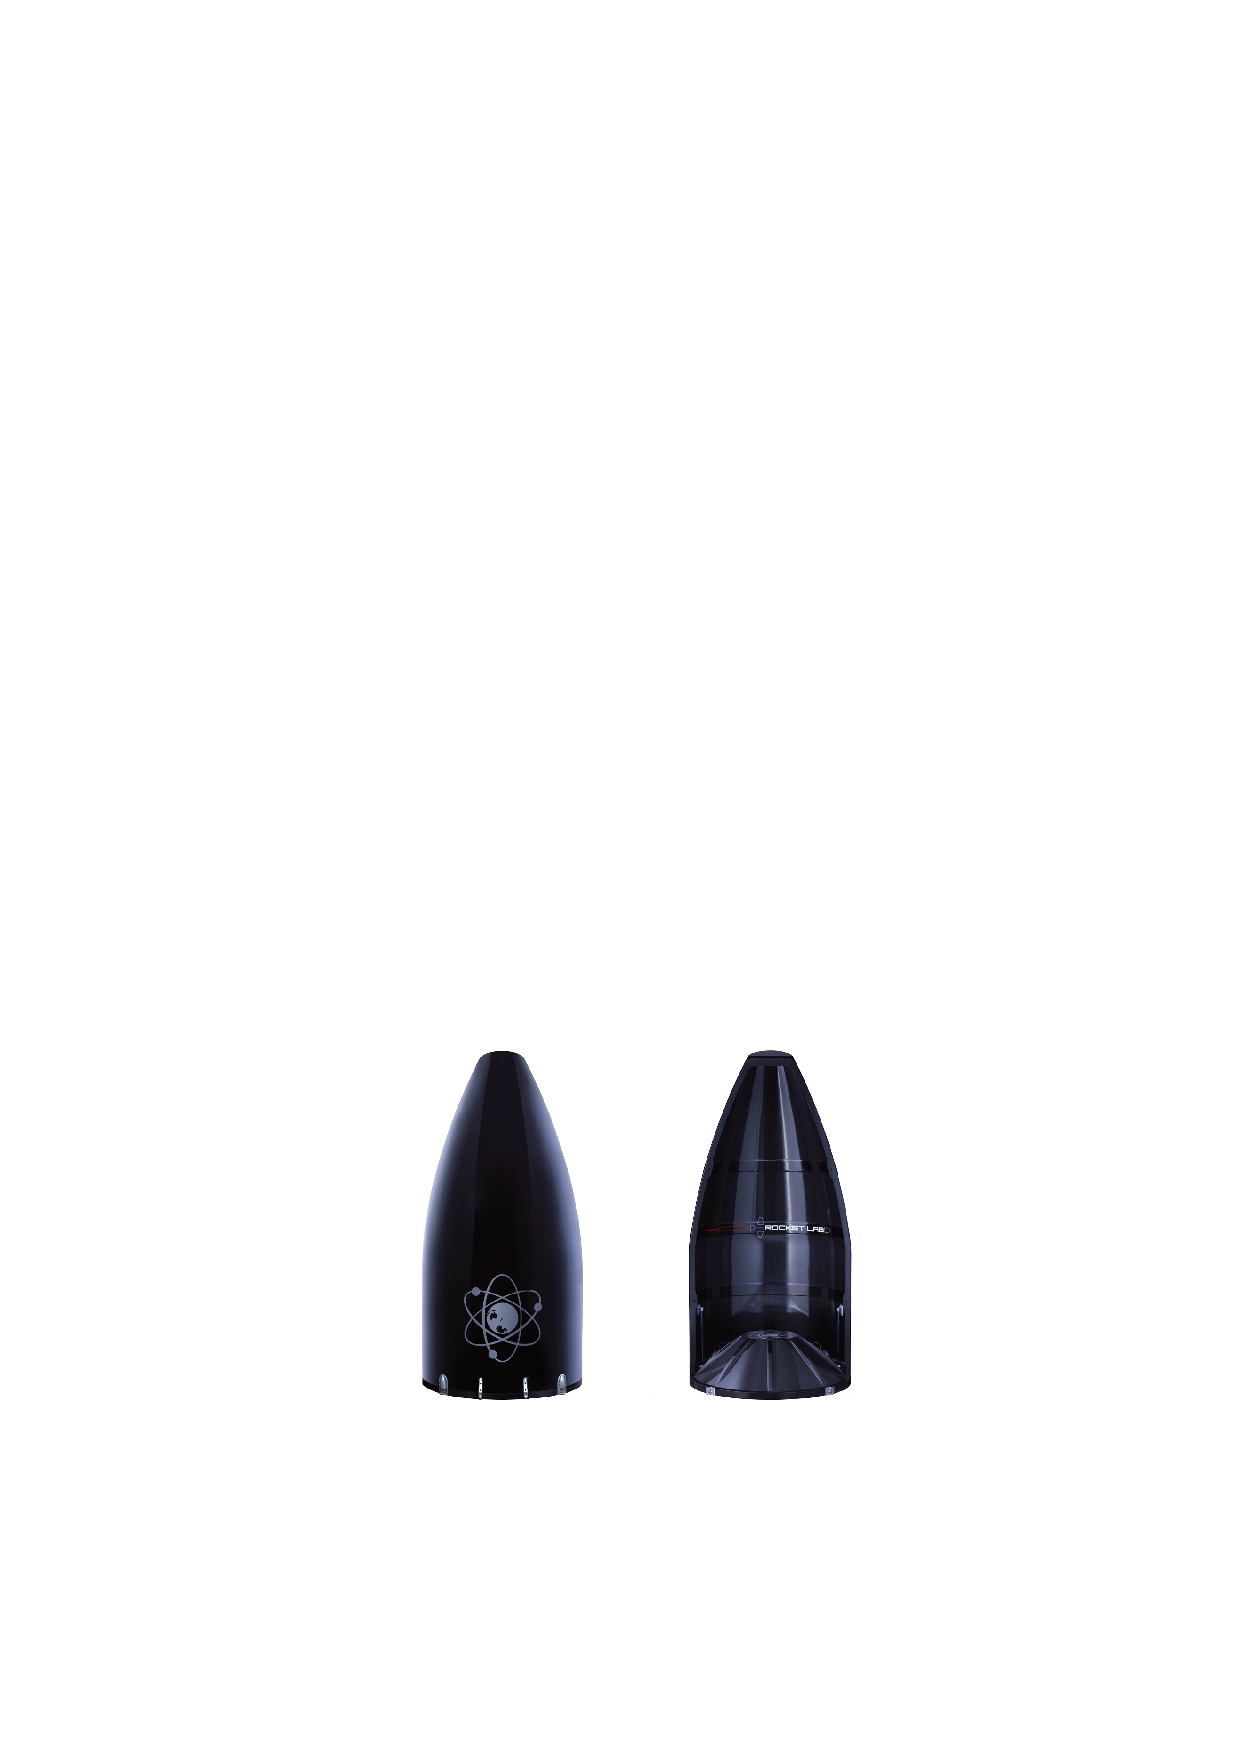
\includegraphics[scale=0.7]{./sections/Constellation_Deployment/S2-Launcher/Images_S2/Picture_3_S2.pdf} 
\caption{Electron Rocket Fairing}
\end{figure}
\newline\newline
\begin{figure}[h!]
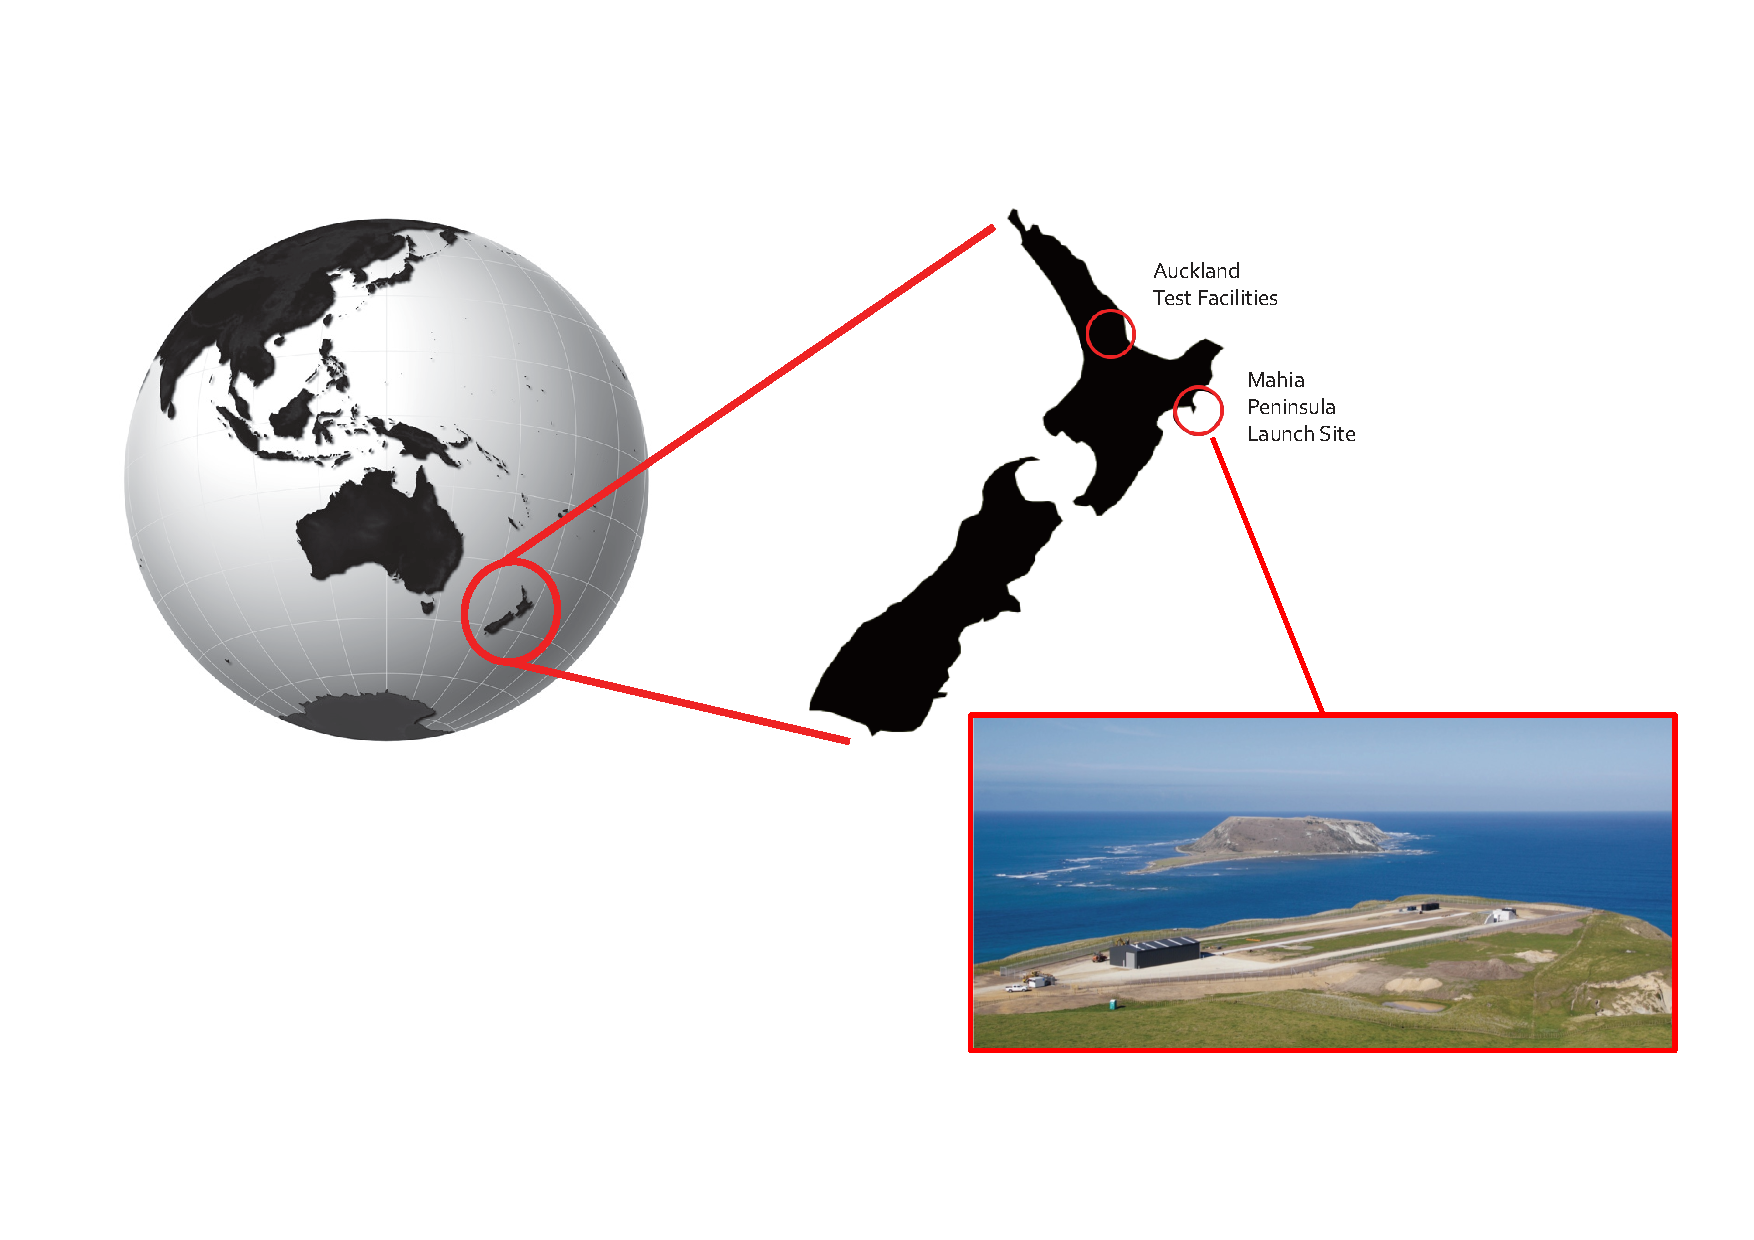
\includegraphics[scale=0.5]{./sections/Constellation_Deployment/S2-Launcher/Images_S2/Picture_4_S2.pdf} 
\caption{Rocket Lab Facilities}
\label{facilities}
\end{figure}